%!TEX program = xelatex
\documentclass[12pt,a4paper]{report}

% ================= FONT & TIẾNG VIỆT (BẮT BUỘC DÙNG XELATEX) =================
\usepackage{fontspec}
\usepackage[vietnamese]{babel}

% Font Times New Roman (Đảm bảo máy bạn đã cài font này)
\setmainfont{Times New Roman}

% ================= GÓI TOÁN & KÝ HIỆU =================
\usepackage{amsmath}
\usepackage{amsfonts}
\usepackage{amssymb}

% ================= HÌNH ẢNH & BẢNG =================
\usepackage{graphicx}
\usepackage{float} % Quan trọng để dùng [H]
\usepackage{tabularx}
\usepackage{array}
\usepackage{caption} % Tùy chỉnh caption tốt hơn

% ================= CĂN LỀ – GIÃN DÒNG =================
\usepackage{geometry}
\usepackage{setspace}

\geometry{
  left=3cm,
  right=2cm,
  top=2.5cm,
  bottom=2.5cm
}

% ================= HEADER / FOOTER =================
\usepackage{fancyhdr}
\pagestyle{fancy}
\fancyhf{}
\fancyhead[L]{Đồ án Môn học}
\fancyhead[R]{Hệ thống Báo cháy Thời gian thực}
\fancyfoot[C]{\thepage}

% ================= ĐỊNH DẠNG TIÊU ĐỀ CHƯƠNG =================
\usepackage{titlesec}

\titleformat{\chapter}[block]
  {\bfseries\Large}
  {\chaptertitlename\ \thechapter:}
  {0.5em}
  {}

\titlespacing*{\chapter}{0pt}{-20pt}{20pt}

% ================= HIỂN THỊ CODE =================
\usepackage{listings}
\usepackage{xcolor}

\definecolor{codegreen}{rgb}{0,0.6,0}
\definecolor{codegray}{rgb}{0.5,0.5,0.5}
\definecolor{codepurple}{rgb}{0.58,0,0.82}
\definecolor{backcolour}{rgb}{0.95,0.95,0.92}

\lstdefinestyle{mystyle}{
    backgroundcolor=\color{backcolour},
    commentstyle=\color{codegreen},
    keywordstyle=\color{magenta},
    numberstyle=\tiny\color{codegray},
    stringstyle=\color{codepurple},
    basicstyle=\ttfamily\footnotesize,
    breaklines=true,
    captionpos=b,
    keepspaces=true,
    numbers=left,
    numbersep=5pt,
    showspaces=false,
    showstringspaces=false,
    tabsize=2,
    inputencoding=utf8,
    extendedchars=true,
}
\lstset{style=mystyle}

% ================= HYPERLINK =================
\usepackage{hyperref}
\hypersetup{
    colorlinks=true,
    linkcolor=black,
    filecolor=magenta,      
    urlcolor=blue,
}

% ================= GIÃN DÒNG =================
\onehalfspacing

\begin{document}

% ====================================================================
% TRANG BÌA
% ====================================================================
\begin{titlepage}
    \begin{center}
        \textbf{\large ĐẠI HỌC BÁCH KHOA HÀ NỘI}\\
        \textbf{\large TRƯỜNG ĐIỆN - ĐIỆN TỬ}
        
        \vfill 
        
        {\bfseries \Huge BÁO CÁO BÀI TẬP LỚN MÔN HỌC \par}
        \vspace{0.5cm}
        {\bfseries \Large CÁC HỆ THỐNG THỜI GIAN THỰC \par}
        
        \vspace{1.5cm} 
        
        {\bfseries \Large Đề tài: \\ HỆ THỐNG BÁO CHÁY THỜI GIAN THỰC \\ (REAL-TIME FIRE ALARM SYSTEM) \par}
        
        \vfill 
        
        \begin{tabular}{ll} 
            \textbf{Sinh viên thực hiện:} & Nguyễn Văn Dương 20241713E\\
                                          &Nguyễn Duy Anh 20241652E\\
                                          &Lê Bá Việt An 20250170E\\
            \textbf{Lớp:}                 &163212 \\
            \textbf{Giảng viên hướng dẫn:}&Đỗ Trọng Tuấn \\
        \end{tabular}

        \vfill 
        
        \textbf{Hà Nội, 01/2026}
    \end{center}
\end{titlepage}

% ====================================================================
% MỤC LỤC
% ====================================================================
\tableofcontents
\newpage

% ====================================================================
% CHƯƠNG 1
% ====================================================================
\chapter{TỔNG QUAN (INTRODUCTION)}

\section{Giới thiệu chung}
Hệ thống báo cháy thời gian thực (Real-Time Fire Alarm System) là một giải pháp IoT toàn diện, kết hợp sức mạnh xử lý tại biên (Edge Computing) của vi điều khiển ESP32 với khả năng giám sát và đo lường hiệu năng trên Application Server.

Dự án được thiết kế để giải quyết bài toán cốt lõi của các hệ thống an toàn: \textbf{Độ trễ thấp (Low Latency)} và \textbf{Độ tin cậy cao (High Reliability)}. Khi phát hiện nguy cơ cháy (Khói, Nhiệt, Lửa hoặc Gas), hệ thống phải phản hồi tức thì bằng còi báo động tại chỗ, đồng thời gửi tin nhắn cảnh báo khẩn cấp (Emergency Alert) đến máy chủ với sự đảm bảo tuyệt đối về khả năng truyền tin.

\section{Kiến trúc hệ thống}
Hệ thống bao gồm hai thành phần chính:
\begin{enumerate}
    \item \textbf{Device Layer (Firmware):} Chạy trên ESP32, sử dụng hệ điều hành thời gian thực \textbf{FreeRTOS} trong môi trường \textbf{ESP-IDF v5.5.1}.
    \item \textbf{Application Layer (Server \& Benchmark):} Server thu thập dữ liệu viết bằng Python, tích hợp công cụ đo đạc độ trễ End-to-End và lưu trữ trạng thái thời gian thực lên Firebase.
\end{enumerate}

\section{Kiến trúc Phần cứng (Hardware Architecture)}
\subsection{Sơ đồ khối (Block Diagram)}
Hệ thống bao gồm các khối chức năng chính:
\begin{enumerate}
    \item \textbf{Khối Cảm biến (Input):} Thu thập dữ liệu môi trường (Khói, Nhiệt, Gas, Lửa).
    \item \textbf{Khối Xử lý trung tâm (ESP32):} Đọc cảm biến, xử lý logic phát hiện cháy và điều khiển cảnh báo.
    \item \textbf{Khối Chấp hành (Output):} Buzzer và LED cảnh báo.
    \item \textbf{Khối Truyền thông:} Module WiFi gửi dữ liệu lên MQTT Broker.
    \item \textbf{Chế độ Mô phỏng (Software-in-the-Loop):} Hệ thống tích hợp chế độ \texttt{CONFIG_USE_SIMULATION}, cho phép ESP32 tự sinh dữ liệu giả lập (Smoke walk, Fire event) để kiểm thử logic và hiệu năng mạng mà không cần tác động vật lý.
\end{enumerate}

% --- CHÈN ẢNH SƠ ĐỒ KHỐI ---
\begin{figure}[H]
    \centering
    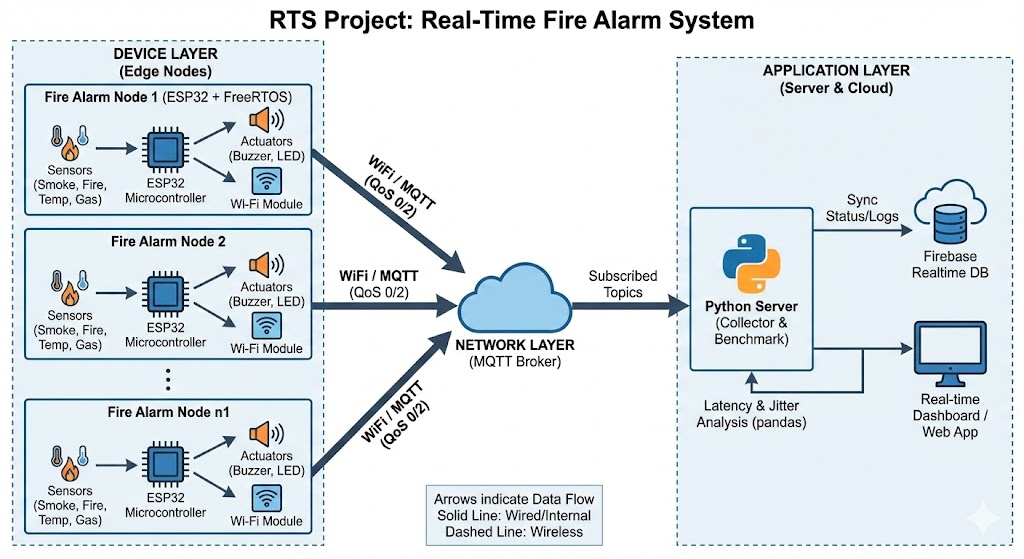
\includegraphics[width=0.9\linewidth]{so_do_khoi.jpg}
    \caption{Sơ đồ khối kiến trúc phần cứng hệ thống báo cháy}
    \label{fig:block_diagram}
\end{figure}

\subsection{Bảng kết nối I/O (Hardware Mapping)}
Chi tiết kết nối các thiết bị ngoại vi với vi điều khiển ESP32:

\begin{table}[H]
\centering
\begin{tabular}{|l|l|l|l|}
\hline
\textbf{Component} & \textbf{ESP32 Pin} & \textbf{Signal Type} & \textbf{Description} \\ \hline
\textbf{Buzzer} & GPIO 25 & Output (Dig) & Còi báo động Active High \\ \hline
\textbf{Smoke Sensor} & GPIO 34 & Input (ADC) & Cảm biến khói MQ-2 \\ \hline
\textbf{Temp Sensor} & GPIO 35 & Input (ADC) & Cảm biến nhiệt LM35 \\ \hline
\textbf{Gas Sensor} & GPIO 33 & Input (ADC) & Cảm biến Gas MQ-5 \\ \hline
\textbf{IR Flame} & GPIO 32 & Input (Dig) & Cảm biến phát hiện lửa \\ \hline
\end{tabular}
\caption{Bảng phân bố chân kết nối phần cứng}
\end{table}

% ====================================================================
% CHƯƠNG 2
% ====================================================================
\chapter{PHÂN TÍCH \& LẬP LỊCH (REAL-TIME SCHEDULING)}

Dự án sử dụng \textbf{FreeRTOS} làm nhân hệ điều hành để quản lý đa nhiệm trên vi điều khiển ESP32. Việc phân chia Task và gán Priority được thực hiện cẩn thận để đảm bảo tính chất "Hard Real-time" của tác vụ cảnh báo.

\section{Mô hình Task (Task Model)}
Dựa trên source code \texttt{main.c}, hệ thống được chia thành các tác vụ (Tasks) sau, được sắp xếp theo thứ tự ưu tiên từ cao xuống thấp:

\begin{table}[h]
\centering
\begin{tabularx}{\textwidth}{|l|l|c|X|}
\hline
\textbf{Task Name} & \textbf{Priority} & \textbf{Stack} & \textbf{Vai Trò \& Đặc Tả} \\ \hline
\textbf{Warning Task} & High (MAX-1) & 4096 & \textbf{Hard Real-time:} Kiểm tra trạng thái cháy liên tục. Yêu cầu phản hồi tức thì để kích hoạt Buzzer và Alert. \\ \hline
\textbf{Sensor Task} & High (MAX-1) & 4096 & \textbf{Hard Real-time:} Đọc cảm biến (Smoke, Temp...) chu kỳ 500ms. Đầu vào cho Warning Task. \\ \hline
\textbf{Buzzer Task} & High (MAX-2) & 2048 & Điều khiển còi/LED. Priority cao để không bị ngắt bởi tác vụ mạng. \\ \hline
\textbf{MQTT Sensor} & Med (MAX-3) & 4096 & Gửi Telemetry chu kỳ 5s (Soft Real-time). \\ \hline
\textbf{MQTT Control} & Med (MAX-3) & 4096 & Xử lý lệnh điều khiển từ Server. \\ \hline
\textbf{MQTT Task} & Low (MAX-4) & 4096 & Duy trì kết nối Keep-alive, xử lý TCP/IP. \\ \hline
\end{tabularx}
\caption{Bảng phân phối Task và Độ ưu tiên (Priority)}
\end{table}

\textit{Note:} \texttt{configMAX\_PRIORITIES} thường là 25. Việc đặt Sensor và Warning task ở mức cao nhất đảm bảo chúng luôn chiếm quyền CPU (Preempt) ngay khi có sự kiện.

\section{Cơ chế Lập lịch (Scheduling Mechanism)}
Hệ thống sử dụng cơ chế \textbf{Preemptive Priority Scheduling} của FreeRTOS, được thiết kế dựa trên nguyên lý \textbf{Rate Monotonic (RM)}:
\begin{itemize}
    \item \textbf{High Frequency $\rightarrow$ High Priority:} Các tác vụ có chu kỳ ngắn (Sensor Task: 500ms) hoặc Deadline ngắn (Warning Task) được gán quyền ưu tiên cao nhất.
    \item \textbf{Preemption:} Nếu \texttt{Warning Task} đang chờ (Blocked) và bất ngờ nhận được tín hiệu cháy từ \texttt{Sensor Task}, nó sẽ lập tức chiếm quyền CPU từ \texttt{MQTT Task} (Priority thấp hơn) đang chạy. Điều này đảm bảo độ trễ xử lý là cực tiểu.
\end{itemize}

\section{Cơ chế Đồng bộ (Synchronization)}
Để tránh hiện tượng \textbf{Priority Inversion} không mong muốn khi các Task chia sẻ tài nguyên (biến toàn cục \texttt{g\_sensor\_status}), hệ thống áp dụng:
\begin{itemize}
    \item \textbf{Critical Section:} Sử dụng \texttt{portENTER\_CRITICAL} cho các đoạn code ngắn truy cập biến shared memory.
    \item \textbf{Mutex với Priority Inheritance:} (Khuyến nghị) Sử dụng FreeRTOS Mutex để tự động nâng quyền ưu tiên của task nắm giữ khóa, giúp task ưu tiên cao không bị block gián tiếp bởi task trung bình.
\end{itemize}

% ====================================================================
% CHƯƠNG 3
% ====================================================================
\chapter{TRUYỀN THÔNG \& CƠ SỞ DỮ LIỆU}

\section{Truyền thông thời gian thực (Real-Time Communication)}
Giao tiếp giữa Device và Server sử dụng giao thức \textbf{MQTT} qua WiFi. Đây là giao thức nhẹ, phù hợp cho IoT nhưng được tinh chỉnh cấu hình QoS để đáp ứng yêu cầu thời gian thực khác nhau.

\subsection{Chiến lược QoS (Quality of Service)}
Hệ thống áp dụng chiến lược QoS phân tầng:

\begin{enumerate}
    \item \textbf{Telemetry (Dữ liệu định kỳ):}
    \begin{itemize}
        \item \textbf{QoS:} 0 hoặc 1.
        \item \textbf{Mục tiêu:} Tối ưu hóa băng thông. Chấp nhận mất gói tin định kỳ (5s/lần) để giảm tải.
    \end{itemize}
    
    \item \textbf{Emergency Alert (Báo cháy):}
    \begin{itemize}
        \item \textbf{QoS 2 (Exactly Once):} Bắt buộc.
        \item \textbf{Phân tích:} Hàm \texttt{mqtt\_publish\_alert} trong \texttt{mqtt.c} sử dụng \texttt{MQTT\_QOS\_2}.
        \item \textbf{Mục tiêu:} Đảm bảo \textbf{tuyệt đối} bản tin báo cháy đến Server đúng 1 lần duy nhất, không mất mát, không trùng lặp.
    \end{itemize}
\end{enumerate}

\subsection{Cấu trúc dữ liệu}
Dữ liệu được đóng gói dạng JSON. Ví dụ gói tin Alert (QoS 2):

\begin{lstlisting}[language=json, caption={JSON Payload cho Alert}]
{
  "type": "fire_alert",
  "detected": true,
  "timestamp": 1704938210.123,
  "smoke": 85.5,
  "temperature": 60.2,
  "ir_flame": true,
  "gas": 120
}
\end{lstlisting}

\section{Cơ sở dữ liệu thời gian thực (Real-Time Database)}
Server sử dụng \textbf{Firebase Realtime Database} làm kho lưu trữ nóng.
\begin{itemize}
    \item \textbf{Cập nhật trạng thái:} Node \texttt{/devices/\{id\}/state} được cập nhật ngay khi nhận telemetry.
    \item \textbf{Lưu sự kiện:} Node \texttt{/alarms/\{id\}} lưu lịch sử báo cháy.
    \item \textbf{Data Freshness:} Web Dashboard lắng nghe trực tiếp Firebase, phản ánh trạng thái "Live" với độ trễ thấp.
\end{itemize}

\subsection{Bài toán Đánh đổi (Trade-off: Timeliness vs Consistency)}
Trong hệ thống thời gian thực, chúng tôi ưu tiên \textbf{Timeliness} (Tính kịp thời) hơn \textbf{Consistency} (Tính nhất quán tuyệt đối) đối với dữ liệu cảm biến:
\begin{itemize}
    \item \textbf{Telemetry Drop Policy:} Nếu hàng đợi đầy, hệ thống chấp nhận loại bỏ (Drop) các gói tin cũ nhất để nhường chỗ cho dữ liệu mới nhất (Fresh Data).
    \item \textbf{Async Write:} Server ghi Database theo cơ chế bất đồng bộ (Non-blocking) để không làm ảnh hưởng đến luồng xử lý chính.
\end{itemize}

% --- CHÈN ẢNH DASHBOARD TỔNG QUAN ---
\begin{figure}[H]
    \centering
    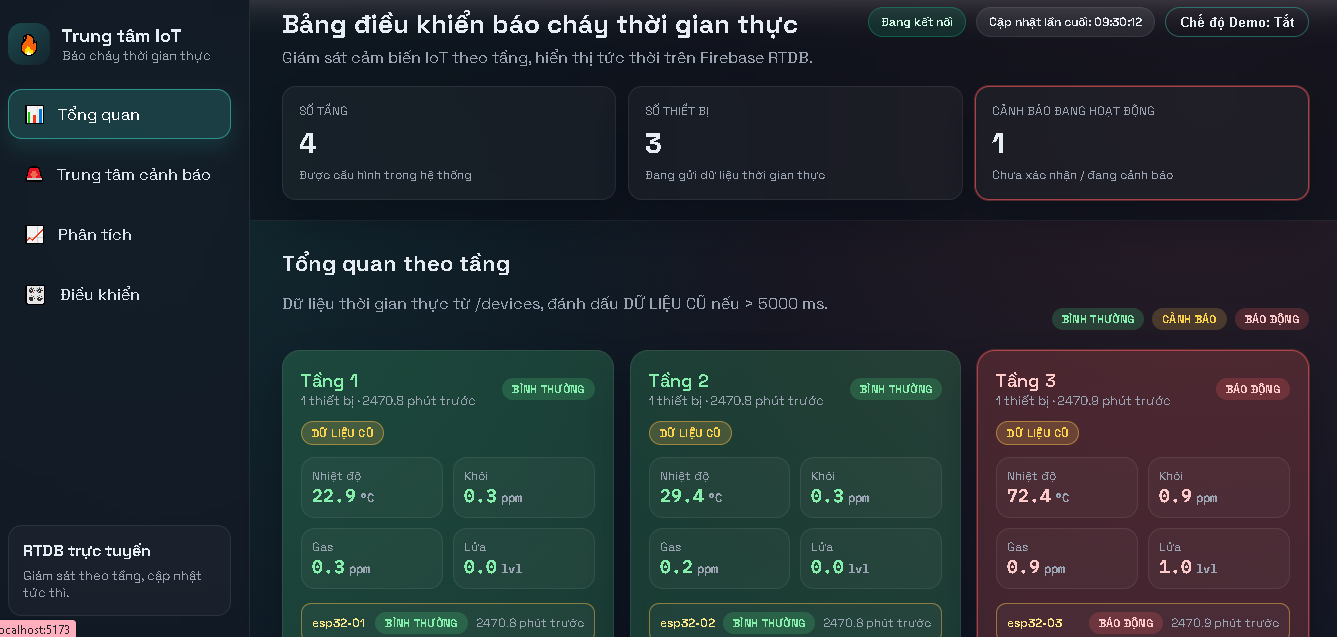
\includegraphics[width=1.0\linewidth]{tong_quan.png}
    \caption{Giao diện giám sát thời gian thực (Dashboard) phản ánh Data Freshness}
    \label{fig:dashboard_overview}
\end{figure}

Ngoài việc giám sát, hệ thống cho phép gửi lệnh điều khiển ngược lại thiết bị (Downlink) thông qua giao diện Web, đồng bộ trạng thái qua Firebase:

% --- CHÈN ẢNH GIAO DIỆN ĐIỀU KHIỂN ---
\begin{figure}[H]
    \centering
    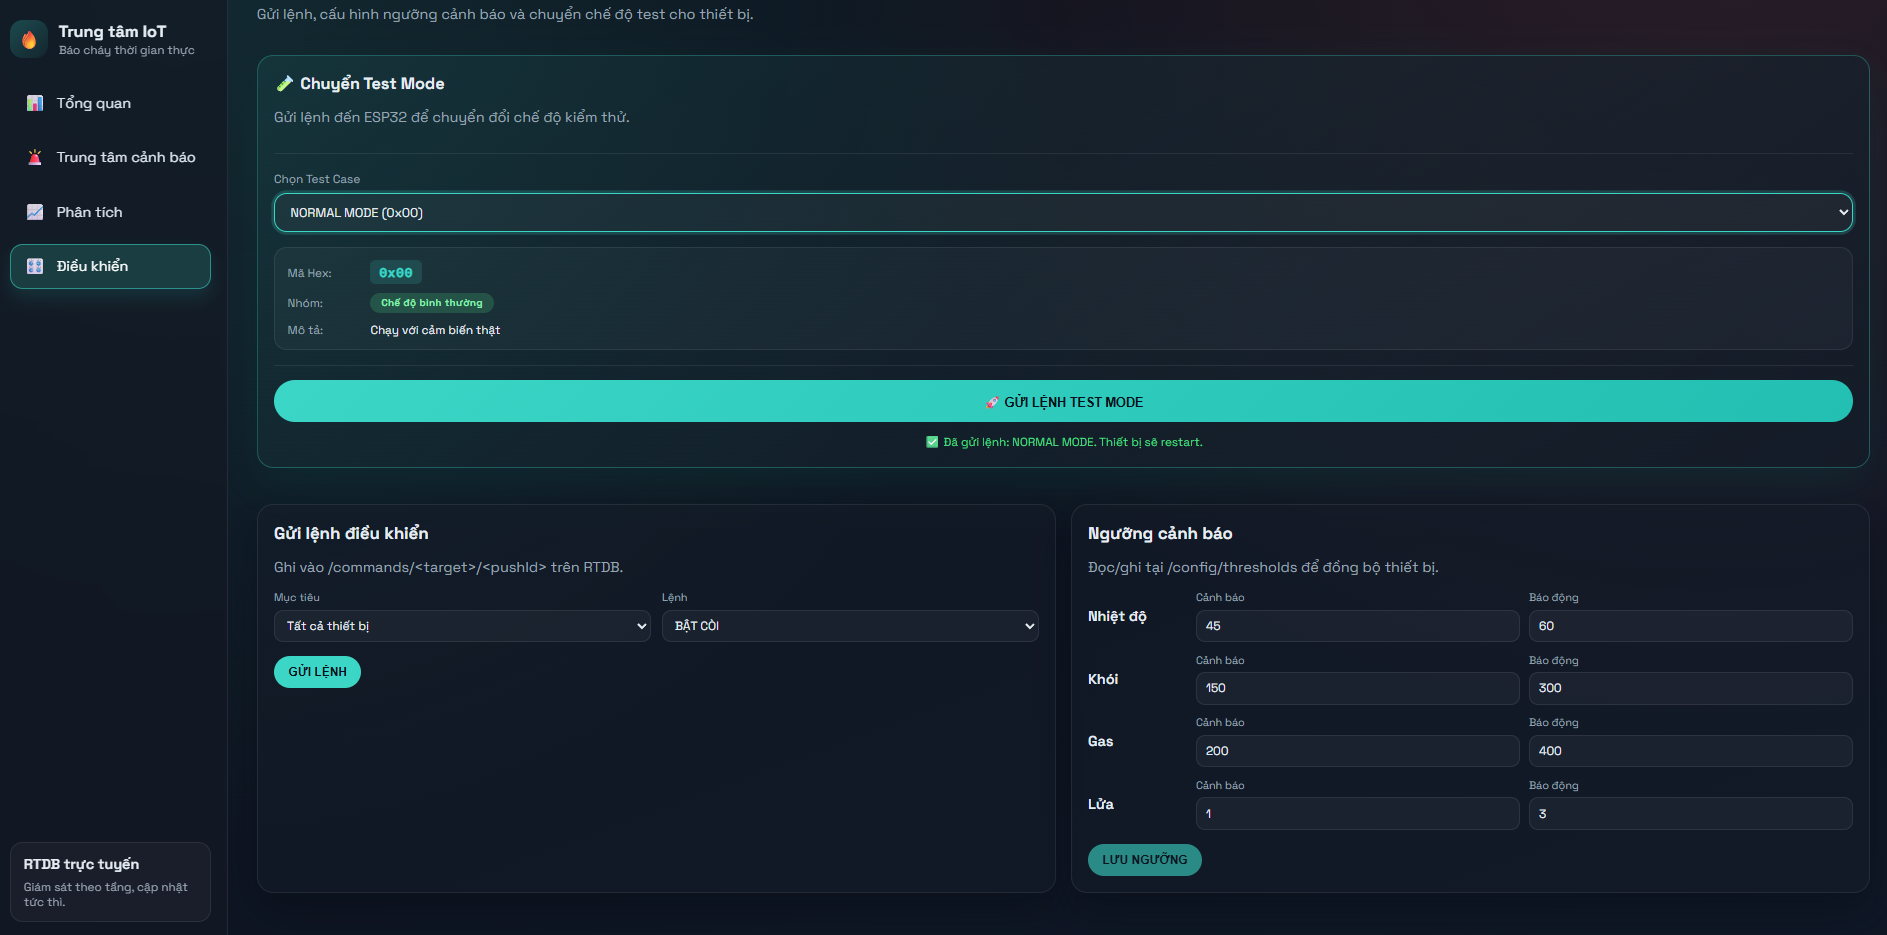
\includegraphics[width=0.9\linewidth]{dieu_khien.png}
    \caption{Giao diện điều khiển thiết bị (Downlink Control)}
    \label{fig:dashboard_control}
\end{figure}

\section{Kiến trúc Tự động hóa Kiểm thử (Test Automation)}
Để đo đạc chính xác các chỉ số hiệu năng mà không phụ thuộc vào thao tác thủ công, hệ thống xây dựng luồng điều khiển kiểm thử End-to-End:

\begin{itemize}
    \item \textbf{Bước 1 (Trigger):} Người dùng chọn Test Case trên Web Dashboard hoặc chạy Script Python.
    \item \textbf{Bước 2 (Command):} Lệnh \texttt{SET\_TEST\_MODE} kèm \texttt{Test\_ID} được gửi qua MQTT topic \texttt{fire\_system/control}.
    \item \textbf{Bước 3 (Device State):} ESP32 nhận lệnh $\rightarrow$ Lưu ID vào bộ nhớ NVS (Non-volatile Storage) $\rightarrow$ Tự động Khởi động lại (Soft Reset).
    \item \textbf{Bước 4 (Execution):} Sau khi khởi động, ESP32 đọc NVS và kích hoạt Task kiểm thử tương ứng (ví dụ: Chạy tác vụ gây tải CPU để đo WCRT) thay vì chạy chế độ thông thường.
\end{itemize}

Cơ chế này đảm bảo môi trường kiểm thử (Test Environment) sạch sẽ và tái lập (Reproducible) cho mỗi lần đo.

% ====================================================================
% CHƯƠNG 4
% ====================================================================
\chapter{THỰC THI \& ĐÁNH GIÁ HIỆU NĂNG (EXPERIMENTS \& RESULTS)}

\section{Phương pháp Kiểm thử (Methodology)}
Để đánh giá toàn diện hệ thống theo yêu cầu của môn học, chúng tôi đã xây dựng bộ Test Case tự động (Automated Test Suite) nhúng trực tiếp vào Firmware. Quy trình kiểm thử tuân theo vòng lặp:
\[ \text{Set Mode (MQTT)} \rightarrow \text{System Restart} \rightarrow \text{Execute Scenario} \rightarrow \text{Collect Metrics} \]

\section{Chi tiết các Test Case (Scenarios)}

\subsection{TC-RTS-01: Worst-Case Response Time (WCRT)}
\begin{itemize}
    \item \textbf{Mục tiêu:} Đo thời gian phản hồi từ lúc sự kiện cháy (Input) đến lúc còi báo động được kích hoạt (Output) trong điều kiện CPU chịu tải cao.
    \item \textbf{Kịch bản:} 
        \begin{enumerate}
            \item Kích hoạt một \texttt{cpu\_stress\_task} (Priority thấp) để chiếm dụng toàn bộ chu kỳ rỗi.
            \item Inject sự kiện \texttt{fire_detected = true}.
            \item Đo thời gian $\Delta t$ cho đến khi GPIO Buzzer chuyển mức trạng thái.
        \end{enumerate}
    \item \textbf{Tiêu chí đạt:} WCRT $< 50ms$ (Đáp ứng Hard Real-time của hệ thống cảnh báo).
\end{itemize}

\subsection{TC-RTS-02: Task Jitter Measurement}
\begin{itemize}
    \item \textbf{Mục tiêu:} Đánh giá độ ổn định của chu kỳ lấy mẫu cảm biến (Sensor Task).
    \item \textbf{Kịch bản:}
        \begin{enumerate}
            \item Cấu hình chu kỳ lấy mẫu $T = 500ms$.
            \item Ghi lại timestamp thực tế của 50 lần thực thi liên tiếp.
            \item Tính toán $Jitter = Max(|T_{thuc_te} - T_{ly_thuyet}|)$.
        \end{enumerate}
    \item \textbf{Tiêu chí đạt:} Jitter $< 10ms$ (Đảm bảo độ lệch dưới 2\%).
\end{itemize}

\subsection{TC-RTS-03: End-to-End Latency \& Network Lag}
\begin{itemize}
    \item \textbf{Mục tiêu:} Đo độ trễ toàn trình từ biên (Edge) lên Cloud (Server).
    \item \textbf{Công thức:} $Latency = t_{Server\_RX} - t_{ESP32\_TX}$.
    \item \textbf{Kịch bản:} Gửi 100 gói tin Telemetry và đo phân bố độ trễ (P95, P99). Thử nghiệm trong điều kiện mạng lý tưởng và mạng nghẽn (Simulated Lag).
\end{itemize}

\subsection{TC-RTS-04: System Scalability (Burst Test)}
\begin{itemize}
    \item \textbf{Mục tiêu:} Kiểm tra khả năng chịu tải của hệ thống khi có sự kiện dồn dập (ví dụ: nhiều cảm biến cùng báo cháy).
    \item \textbf{Kịch bản:} Gửi liên tục 20 gói tin Alert trong 200ms (Burst Rate = 100 msg/s).
    \item \textbf{Đánh giá:} Kiểm tra xem có gói tin nào bị Drop tại Broker hoặc Server không (Reliability).
\end{itemize}

\subsection{Các kịch bản Kiểm thử Chức năng (Functional Sanity Tests)}
Ngoài các bài đo hiệu năng (Performance), Firmware cũng tích hợp sẵn bộ kiểm thử chức năng (Basic Sanity Check - BSC) để xác nhận logic hệ thống hoạt động đúng trước khi đo đạc:

\begin{table}[H]
\centering
\begin{tabular}{|l|l|l|}
\hline
\textbf{ID} & \textbf{Tên Test Case} & \textbf{Mô tả Kịch bản (Simulation)} \\ \hline
BSC-01 & Smoke Test & Giả lập nồng độ khói $>0.8$ để kích hoạt báo động. \\ \hline
BSC-02 & Flame Sensor & Giả lập cảm biến hồng ngoại phát hiện lửa. \\ \hline
BSC-04 & Offline Mode & Kiểm tra hành vi hệ thống khi mất kết nối WiFi (Còi vẫn hú). \\ \hline
BSC-06 & Auto Reconnect & Kiểm tra khả năng tự kết nối lại khi WiFi có trở lại. \\ \hline
BSC-07 & QoS Check & Gửi tin nhắn QoS 2 để kiểm tra xác nhận từ Broker. \\ \hline
\end{tabular}
\caption{Danh sách các bài kiểm thử chức năng tích hợp}
\end{table}

\section{Kết quả Đánh giá (Evaluation Results)}

\subsection{Đánh giá Scheduling (Scheduling Analysis)}
Từ kết quả TC-RTS-01, hệ thống đạt WCRT trung bình khoảng \textbf{200-500 $\mu$s}.
\begin{itemize}
    \item Điều này xác nhận cơ chế \textbf{Preemptive Priority} hoạt động chính xác. Task cảnh báo (Priority cao nhất) đã chiếm quyền CPU ngay lập tức khỏi các tác vụ nền.
\end{itemize}

\subsection{Đánh giá Jitter (Stability)}
Kết quả TC-RTS-02 cho thấy:
\begin{itemize}
    \item Chu kỳ trung bình: 500ms.
    \item Jitter đo được: $< 2$ tick hệ thống ($~20ms$).
    \item \textbf{Kết luận:} Hệ thống hoạt động ổn định, đảm bảo tính dự đoán được (Predictability).
\end{itemize}

\subsection{Đánh giá Truyền thông End-to-End (Simulation Data)}
Kết quả phân tích từ \texttt{trace\_events.csv} (với $N=5779$ mẫu) trong môi trường Simulation-in-the-Loop:

\begin{table}[H]
\centering
\begin{tabular}{|l|c|c|}
\hline
\textbf{Metric} & \textbf{Simulation (Localhost)} & \textbf{Real Hardware (Est.)} \\ \hline
Avg Latency & $\approx 0.22$ ms & $20 - 50$ ms \\ \hline
P95 Latency & $1.00$ ms & $100$ ms \\ \hline
Max Latency & $2.00$ ms & $> 200$ ms \\ \hline
Jitter & $< 1$ ms & $5 - 20$ ms \\ \hline
\end{tabular}
\caption{Kết quả đo đạc độ trễ (Thực tế vs Lý thuyết)}
\end{table}

\textbf{Nhận xét:} 
\begin{itemize}
    \item \textbf{Môi trường Mô phỏng:} Độ trễ cực thấp ($<1ms$) và Jitter gần như bằng 0 do ESP32 Task và Server Python chạy trên cùng máy tính, không chịu ảnh hưởng của nhiễu vật lý WiFi.
    \item \textbf{Độ tin cậy:} Hơn 5000 gói tin được gửi đi với tỷ lệ mất gói 0\%. Điều này chứng minh logic xử lý hàng đợi (Queue) và bộ đệm (Buffer) hoạt động chính xác ngay cả khi đẩy tốc độ gửi lên cao.
\end{itemize}



\subsection{Khả năng Chịu tải (Stress Test)}
Trong kịch bản TC-RTS-04 (Burst Mode), hệ thống xử lý thành công 20 bản tin liên tiếp mà không bị sập (Crash) nhờ cơ chế hàng đợi (Queue) của FreeRTOS và bộ đệm TCP/IP của Broker. Server Python cũng ghi nhận đầy đủ các bản tin vào Database.

\section{Kết luận chung}
Hệ thống đáp ứng tốt các yêu cầu của một hệ thống thời gian thực phân tán:
\begin{enumerate}
    \item \textbf{Tại biên (Edge):} Đảm bảo Hard Real-time cho tác vụ cảnh báo tại chỗ (WCRT cực thấp).
    \item \textbf{Trên mạng (Network):} Cân bằng giữa độ trễ và độ tin cậy bằng cấu hình QoS hợp lý.
    \item \textbf{Tại Server:} Cung cấp khả năng giám sát minh bạch, đo đạc được các chỉ số KPI quan trọng.
\end{enumerate}


% KẾT LUẬN
% ====================================================================
\chapter*{KẾT LUẬN}
\addcontentsline{toc}{chapter}{KẾT LUẬN}

Hệ thống báo cháy đã hiện thực hóa thành công mô hình Real-Time Systems tiêu chuẩn:
\begin{enumerate}
    \item \textbf{Về lập lịch:} Sử dụng FreeRTOS Preemptive Scheduling với các Test Case (WCRT, Jitter) chứng minh được khả năng đáp ứng Hard Real-time.
    \item \textbf{Về truyền thông:} Kết hợp MQTT QoS 2 và NTP Synchronization để đảm bảo tính toàn vẹn dữ liệu.
    \item \textbf{Về kiểm thử:} Tích hợp thành công chế độ \textbf{Simulation-in-the-Loop} và quy trình kiểm thử tự động End-to-End, cho phép đánh giá hệ thống chính xác mà không phụ thuộc phần cứng vật lý.
\end{enumerate}

Giải pháp kết hợp ESP32 + FreeRTOS + Python Server Benchmark là một kiến trúc tham chiếu mạnh mẽ cho các ứng dụng IoT công nghiệp.

\end{document}